\documentclass{article}
\usepackage[%
    left=0.5in,%
    right=0.5in,%
    top=0.5in,%
    bottom=0.5in,%
]{geometry}%
\usepackage{minitoc}
\usepackage{multicol}
\usepackage{graphicx}
\usepackage{fixltx2e}
\usepackage{hyperref}
\usepackage{hyperref}
    \hypersetup{ colorlinks = true, linkcolor = blue }
\usepackage{blindtext}

\graphicspath{ {./} }

\newcommand{\inlinecode}[2]{\colorbox{lightgray}{\lstinline
[language=#1]$#2$}}
\newcommand{\worddef}[1]{\hyperref[sec:reference]{\textit{#1}}}

\begin{document}

\section{File system consistency}
\begin{flushleft}
Journaling \textbf{heavily reduces} the probability of having inconsistencies in a file system. In case of crash, the log \textbf{stores} what operations \textbf{were not run}. However, it can still be possible to get some \textbf{inconsistencies} (e.g. data blocks weren’t flushed to the drive, typical case on USB drives!). This can be problematic, in particular for \textbf{structural blocks} such as i-nodes, directories, and free lists. System utilities are available to restore file systems, e.g.: (Scandisk, FSCK) There are two main consistency checks: \textbf{block} and \textbf{directory}.
\end{flushleft}

\subsection{Block consistency}
\begin{flushleft}
Block consistency checks whether blocks are \textbf{assigned/used} the correct way. Block consistency is checked by building two tables:
\begin{itemize}
	\item Table one counts how often a \textbf{block} is present in a \textbf{file} (based on the i-nodes)
	\item Table two counts how often a \textbf{block} is present in the \textbf{free list} 
\end{itemize}
A consistent file system has a 1 in either of the tables for each block. Typically, this is a \textbf{very slow} process, taking even hours (and running with the partition unmounted)
\end{flushleft}

\subsubsection{Restoring}
\begin{flushleft}
\begin{itemize}
	\item A \textbf{missing block}: it does not exist in any of the tables add it to the \textbf{free list}.
	\item A block is \textbf{double counted} in the free list (“disaster” waiting to happen) \textbf{re-build} the free list.
	\item A block is present in two or more files.
	\begin{itemize}
		\item Removing one file results in the adding the block to the free list
		\item Removing both files will result in a double entry in the free list
		\item Solution: use new free block and copy the content (the file is still likely to be damaged)
	\end{itemize}
\end{itemize}
\bigskip
\textbf{FSCK Algorithm:}
\begin{itemize}
	\item Iterate through all the i-nodes - retrieve the blocks - increment the counters
	\item Iterate through the free list - increment counters for free blocks
\end{itemize}
\end{flushleft}

\subsection{Restoring I-node consistency}
\begin{flushleft}
Checking the directory system: are the \textbf{i-node counts correct}? Where can it go wrong?:
\begin{itemize}
	\item I-node counter is \textbf{higher} than the number of directories containing the file
	\begin{itemize}
		\item Removing the file will reduce the i-node counter by 1.
		\item Since the counter will remain larger than 1, the i-node / disk space \textbf{will not be released} for future use
	\end{itemize}
	\item I-node counter is \textbf{less} than the number of directories containing the file
	\begin{itemize}
		\item Removing the file will (\textbf{eventually}) set the i-node counter to 0 whilst the file is \textbf{still referenced}
		\item The file / i-node will be released, even though the file was \textbf{still in use}
	\end{itemize}
\end{itemize}
 Recurse through the directory hierarchy - \textbf{Increment} file specific counters - I.e. each file is associated with one counter.\\
 One file may appear in multiple directories - Compare the file and i-node counters - Correct if necessary
\end{flushleft}
\begin{center}
	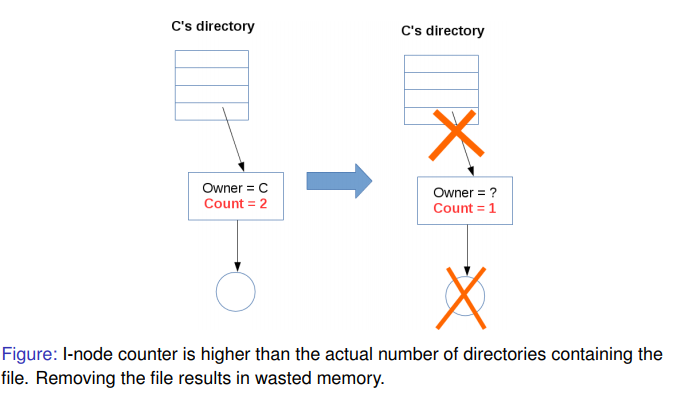
\includegraphics[scale=0.3]{i_node_constency_higher.png}
	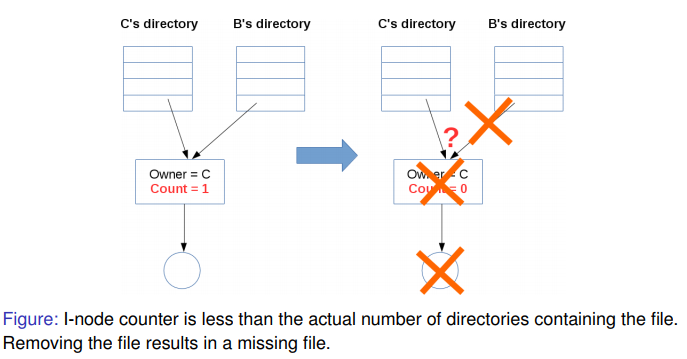
\includegraphics[scale=0.3]{i_node_consistency_lower.png}
\end{center}

\section{File system}
\subsection{Defragmentation}
\begin{flushleft}
At the beginning, all free disk space is in a \textbf{single contiguous} unit. After a while, creating and removing files, a disk may end up badly \textit{fragmented} (holes and file all over the place). Defrag utilities make file blocks \textbf{contiguous} (very slow operation), and free space in one or more large \textbf{contiguous regions} on the disk. Windows users should run this regularly, except on SSDs. Linux (\textbf{ext2/3}) suffers less from fragmentation. Defragmentating SSD is \textbf{counter-productive} (No gain in performance and SSDs wear out).
\end{flushleft}

\subsection{History}
\begin{itemize}
	\item \textbf{Minix file system}: the maximum file size was 64MB and file names were limited to 14 characters.
	\item The “extended file system” (\textbf{extfs}): file names were 255 characters and the maximum file size was 2 GB.
	\item The \textbf{“ext2}” file system: larger files, larger file names, better performance.
	\item The “\textbf{ext3-4}” file system: journaling etc.
\end{itemize}

\subsection{The extended 2 file system (ext2)}
\begin{flushleft}
The second extended file system (\textbf{ext2}) is one of the \textbf{most popular} file systems in Linux. The main goals:
\begin{itemize}
	\item Improve the performance of MINIX and extfs file systems, distributing directories evenly over the disk.
	\item Allow greater \textbf{file names} and \textbf{sizes}, improving directory implementation.
\end{itemize}
\begin{center}
	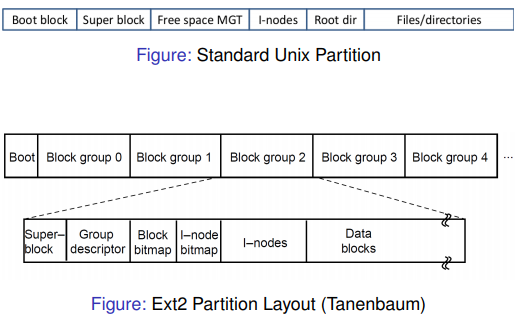
\includegraphics[scale=0.4]{ext2_vs_reg.png}
\end{center}
An ext2 partition is split into several \textbf{block groups} to:
\begin{itemize}
	\item \textbf{Reduce fragmentation} by storing i-nodes and files, and parent directories and files in the \textbf{same block} group if possible.
	\item \textbf{Reduce} seek times and \textbf{improve} performance
	\item All block groups have the \textbf{same size} and are stored \textbf{sequentially} (which allows direct indexing)
\end{itemize}
\end{flushleft}

\pagebreak
\subsection{Directory entries}
\begin{itemize}
	\item The \textbf{superblock} contains file system information (e.g. the number of i-nodes, disk blocks)
	\item The \textbf{group descriptor} contains \textbf{bitmap locations}, the number of \textbf{free blocks}, \textbf{i-nodes} and \textbf{directories}
	\item A \textbf{data block bitmap} and \textbf{i-node bitmap}, used to keep track of free disk blocks and i-nodes (Unix uses lists)
	\item A \textbf{table} of i-nodes containing file and disk block information
	\item \textbf{Data blocks} containing file and directory blocks
\end{itemize}
\begin{flushleft}
Every directory entry contains the following fixed-length fields:
\begin{itemize}
	\item i-node number
	\item Entry size in bytes
	\item Type field, i.e. file, directory, special file, etc.
	\item File name length in bytes
	\item And then, the file name itself (of variable-length).
\end{itemize}
Directories are searched \textbf{linearly} (i.e. they are \textbf{unsorted}) and a \textbf{cache is maintained} for recently accessed items.
\end{flushleft}
\begin{center}
	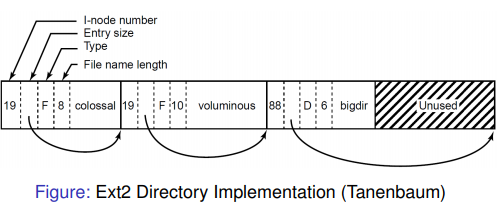
\includegraphics[scale=0.6]{directory_implementation.png}
\end{center}
\begin{itemize}
	\item File names up to \textbf{255 characters}
	\item \textbf{File lookups} are similar to the Unix file system.
	\item The i-node structure is similar to the Unix i-nodes
	\begin{itemize}
		\item 12 block addresses are contained in the i-node
		\item Single, double and triple indirect blocks are used
		\item With a blocks of 1KB, this scheme can handle file sizes of 16GB.
		\item If block size is 8KB, it could support file sizes up to 64TB.
	\end{itemize}
\end{itemize}

\subsection{Ext3}
\begin{flushleft}
When making changes to an \textbf{Ext2} file system, files are ideally written immediately to prevent inconsistency: This generates \textbf{significant} head movement. Ext2 File system is more suitable for \textbf{flash disks} (no journal).\\
\textbf{Ext3} builds upon the Ext2 file system by adding: \textbf{Tree based structures} for directory files to facilitate indexing (HTrees). \textbf{Journaling capabilities}
\end{flushleft}

\pagebreak
\section*{Reference section} \label{sec:reference}
\begin{description}
	\item[placeholder] \hfill \\
\end{description}
\end{document}
